\subsection{Evaluating Compound Expressions}
\label{Section 1.1.3}

One of our goals in this chapter is to isolate issues about thinking
procedurally.  As a case in point, let us consider that, in evaluating compound
expressions, the interpreter is itself following a procedure.

To evaluate a compound expression, do the following:

\begin{enumerate}

\item
Evaluate the subexpressions of the compound expression.

\item
Apply the operation denoted by the operator to the arguments that are the
values of the operands.

\end{enumerate}

\noindent
Stated that way the rule says nothing about where the operator was written, and
it need not.  Before Python evaluates anything it reads what we typed and
builds a tree from it: each compound expression becomes a node holding its
operator and its operands, and each operand is itself such a node, or a number,
or a name.  Infix is how we write the tree down; it is not what the interpreter
works on.  If we were to write out the tree Python builds for \code{2 + 4 * 6}
in the notation of the original, we would get exactly

\begin{syntaxForm}
(+ 2 (* 4 6))
\end{syntaxForm}

\noindent
which is to say that the difference between the two languages here is a
difference of notation and not of substance.  Lisp writes the tree down
directly, which is why a Lisp program looks the way it does; Python writes it
down in the order we are used to from arithmetic and reconstructs the tree when
it reads the line.  Both interpreters then have the same thing in hand, and the
rule above applies to it unchanged.

Even this simple rule illustrates some important points about processes in
general.  First, observe that the first step dictates that in order to
accomplish the evaluation process for a compound expression we must first
perform the evaluation process on each of its subexpressions.  Thus, the
evaluation rule is \newterm{recursive} in nature; that is, it includes, as one
of its steps, the need to invoke the rule itself.\footnote{The original pauses
here to observe that it seems strange for the rule to evaluate the operator, as
that can only be a symbol such as \code{+} standing for a built-in procedure,
and promises that it will later be useful for the operator to be something we
compute.  Python does not evaluate its operators at all: \code{+} is built-in
syntax, and there is nothing to look up.  The promise is kept, but in another
form, and we shall come to it in \link{Section 1.3}.}

Notice how succinctly the idea of recursion can be used to express what, in the
case of a deeply nested expression, would otherwise be viewed as a rather
complicated process.  For example, consider the expression evaluating

\begin{codeBlock}
>>> (2 + 4 * 6) * (3 + 5 + 7)
~\textit{390}~
\end{codeBlock}

If we isolate all the binary operations, we can rewrite it as

\begin{codeBlock}
>>> ((2 + (4 * 6)) * ((3 + 5) + 7))
~\textit{390}~
\end{codeBlock}

\noindent
Notice that there are five grouping of parentheses and the calculation requires that the evaluation rule be applied to five different compound
expressions.  We can obtain a picture of this process by representing the
expression in the form of a tree, as shown in \link{Figure 1.1}.  Each compound
expression is represented by a node with branches corresponding to the operator
and the operands stemming from it.  The terminal nodes (that is, nodes with no
branches stemming from them) represent either operators or numbers.  Viewing
evaluation in terms of the tree, we can imagine that the values of the operands
percolate upward, starting from the terminal nodes and then combining at higher
and higher levels.  In general, we shall see that recursion is a very powerful
technique for dealing with hierarchical, treelike objects.  In fact, the
``percolate values upward'' form of the evaluation rule is an example of a
general kind of process known as \newterm{tree accumulation}.\footnote{Five,
where the original has four, and the tree is correspondingly one level deeper
on the right.  The original writes \code{(+ 3 5 7)}, one application of
\code{+} to three operands; Python has no such form, and \code{3 + 5 + 7} is
two applications of \code{+} to two.  It is the same arithmetic and a different
tree.}

% figure 1.1
\begin{imageFigure}{Tree representation, showing the value of each
  subexpression.}
  % The evaluation tree for (2 + 4 * 6) * (3 + 5 + 7), used in Section 1.1.3.
%
% Drawn rather than vendored because upstream's figure_1.1g is the tree for the
% Lisp expression, and Python's differs in exactly one way: arity. Lisp's
% (+ 3 5 7) is ONE application of + to three operands, so upstream's node has
% three operand branches. Python's 3 + 5 + 7 is (3 + 5) + 7 -- two binary
% applications -- so that subtree is one level deeper, with an intermediate 8.
%
% Everything else is deliberately the same as upstream's, including drawing the
% operator as a branch rather than as a label on the node: Python's parse tree
% really does hold the operator as a child (ast.iter_child_nodes on a BinOp
% yields its operator), so the two figures should be directly comparable.
%
% Every value in upstream's figure survives unchanged: 390, 26, 24, 15.

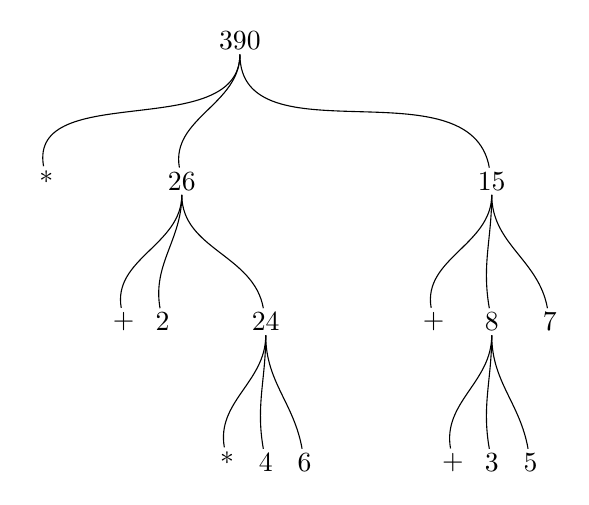
\begin{tikzpicture}[
  x = 0.82cm, y = 1.05cm,
  every node/.style = {inner sep=1.5pt, font=\normalsize},
  branch/.style     = {draw, thin},
]

% level 0
\node (v390) at (-2.4,  0.0) {390};
% level 1
\node (o0)   at (-5.4, -1.7) {*};
\node (v26)  at (-3.3, -1.7) {26};
\node (v15)  at ( 1.5, -1.7) {15};
% level 2
\node (o1)   at (-4.2, -3.4) {+};
\node (n2)   at (-3.6, -3.4) {2};
\node (v24)  at (-2.0, -3.4) {24};
\node (o2)   at ( 0.6, -3.4) {+};
\node (v8)   at ( 1.5, -3.4) {8};
\node (n7)   at ( 2.4, -3.4) {7};
% level 3
\node (o3)   at (-2.6, -5.1) {*};
\node (n4)   at (-2.0, -5.1) {4};
\node (n6)   at (-1.4, -5.1) {6};
\node (o4)   at ( 0.9, -5.1) {+};
\node (n3)   at ( 1.5, -5.1) {3};
\node (n5)   at ( 2.1, -5.1) {5};

\foreach \p/\c in {v390/o0, v390/v26, v390/v15,
                   v26/o1, v26/n2, v26/v24,
                   v15/o2, v15/v8, v15/n7,
                   v24/o3, v24/n4, v24/n6,
                   v8/o4,  v8/n3,  v8/n5}
  \draw[branch] (\p) to[out=-90, in=100] (\c);

\end{tikzpicture}

\end{imageFigure}

Next, observe that the repeated application of the first step brings us to the
point where we need to evaluate, not compound expressions, but primitive
expressions such as numerals, built-in operators, or other names.  We take care
of the primitive cases by stipulating that

\begin{itemize}
\item
the values of numerals are the numbers that they name,

\item
built-in operators stand for the machine instruction sequences that carry out
the corresponding operations, and

\item
the values of other names are the objects associated with those names in the
environment.
\end{itemize}

\noindent
The key point to notice is the role of the environment in determining the
meaning of the symbols in expressions.  In an interactive language such as
Python, it is meaningless to speak of the value of an expression such as
\code{x + 1} without specifying any information about the environment that
would provide a meaning for the symbol \code{x}.\footnote{The original says
``or even for the symbol \code{+},'' and for Lisp that is so: \code{+} is a
name like any other, and could in principle be bound to something else.  In
Python it could not.  This is the one place in this section where the two
languages genuinely part company, and we take it up in
\link{Section 1.1.4}.} As we shall see in \link{Chapter 3}, the general notion
of the environment as providing a context in which evaluation takes place will
play an important role in our understanding of program execution.

Notice that the evaluation rule given above does not handle definitions.  For
instance, evaluating \code{x = 3} does not apply \code{=} to two arguments, one
of which is the value of the symbol \code{x} and the other of which is 3, since
the purpose of the \code{=} is precisely to associate \code{x} with a value.
(That is, \code{x = 3} is not a compound expression.)

In Lisp, such exceptions to the general evaluation rule are called
\newterm{special forms}.  Python draws the line in a different place and gives
it a different name: \code{x = 3} is not an expression at all but a
\newterm{statement}, and statements are a separate category of thing with their
own rules.  Each has its own rule, whatever we call them, and the various kinds
of expressions and statements, each with its associated rule, constitute the
syntax of the programming language.  Here the two languages differ as much as
they differ anywhere.  Lisp has a very simple syntax: the evaluation rule can
be described by a simple general rule together with specialized rules for a
small number of special forms.  Python's syntax is large, and much of what a
Python programmer knows is knowledge of it.\footnote{Special syntactic forms
that are simply convenient alternative surface structures for things that can
be written in more uniform ways are sometimes called \newterm{syntactic sugar},
to use a phrase coined by Peter Landin.  In comparison with users of other
languages, Lisp programmers, as a rule, are less concerned with matters of
syntax.  This disdain for syntax is due partly to the flexibility of Lisp,
which makes it easy to change surface syntax, and partly to the observation
that many ``convenient'' syntactic constructs, which make the language less
uniform, end up causing more trouble than they are worth when programs become
large and complex.  In the words of Alan Perlis, ``Syntactic sugar causes
cancer of the semicolon.''  The reader may judge for themselves how the remark
sits in a language that has semicolons and asks you not to use them.}
